% Informe del laboratorio 3: control de versiones con Git/GitHub y modelo relacional (cierre de la fase 1)
% Compilar desde esta carpeta: pdflatex informe_lab03.tex (dos veces)
\documentclass[a4paper,11pt]{article}
% Preámbulo común de los informes de laboratorio (II/2026). Se incluye desde laboratorios/labNN_*/
%   % Preámbulo común de los informes de laboratorio (II/2026). Se incluye desde laboratorios/labNN_*/
%   % Preámbulo común de los informes de laboratorio (II/2026). Se incluye desde laboratorios/labNN_*/
%   \input{../informe_comun}
\input{../../gemelo-digital/manual/estilo_manual}
\input{../../gemelo-digital/manual/tecnico/macros}
\graphicspath{{../../documentacion/planos_isa/pid/}{../../documentacion/planos_isa/electrico/}{../../documentacion/manuales_inversa/}
  {../../database/mockups/}{../../database/documentacion/}{../../database/modelo/}{../../database/interfaz/}
  {../../gemelo-digital/manual/img/}{../../modelo-3d/informe/figuras/}{../../modelo-3d/levantamiento/}{../../../../global/fotos-planta/}{../figuras/}}
\usepackage{pdflscape}
\lstset{showstringspaces=false}
% plano A3 en una página apaisada: \plano[página]{archivo}{leyenda}
\newcommand{\plano}[3][1]{\begin{landscape}\begin{figure}[p]\centering\includegraphics[page=#1, width=\linewidth, height=0.86\textwidth, keepaspectratio]{#2}\caption{#3}\end{figure}\end{landscape}}
\setlength{\headheight}{14pt}
\newcommand{\nlab}{}
\newcommand{\tlab}{}
\lhead{\small Brazo XK-JS1-1 · Informe del laboratorio \nlab}
\rhead{\small UMSA · II/2026}

% \portada{número}{título}{inicio}{entrega}{semanas}
\newcommand{\portada}[5]{%
\renewcommand{\nlab}{#1}%
\begin{titlepage}
\centering
\vspace*{0.6cm}
{\large Universidad Mayor de San Andrés · Facultad de Ingeniería\par}
{\large Carrera de Ingeniería Electrónica\par}
\vspace{0.8cm}
{\color{naranja!80!black}\rule{\linewidth}{1.5pt}\par}
\vspace{0.3cm}
{\Large Informe del Laboratorio Integrado Nº #1\par}
\vspace{0.2cm}
{\huge\bfseries #2\par}
\vspace{0.3cm}
{\color{naranja!80!black}\rule{\linewidth}{1.5pt}\par}
\vspace{0.8cm}
{\large Planta: brazo robótico XK-JS1-1 de 4 grados de libertad\par}
\vspace{0.3cm}
{\large ETN-902 Sistemas de Control II · ETN-1034 Aplicación de Técnicas de Control · ETN-1000 Bases de Datos\par}
\vspace{1cm}
\begin{tabular}{rl}
\textbf{Docente:} & Ing. Jorge Antonio Nava Amador\\
\textbf{Auxiliares:} & Limber Ajnota · Fabián Plata · Franz Choque\\
\textbf{Inicio de trabajo:} & #3\\
\textbf{Entrega:} & #4 (#5)\\
\end{tabular}
\vspace{1cm}

\begin{tabular}{ll}
\multicolumn{2}{l}{\textbf{Escuadra del brazo de 4 GDL}}\\[2pt]
Control (ETN-902 / ETN-1034): & Gabriel Andres Gomez Calla\\
 & Jose Lenin Mamani Choque\\
 & Miguel Alejandro Lima Huarachi\\
 & Román Abner Machicado Arequipa\\[2pt]
Cómputo (ETN-1000): & Miguel Alejandro Lima Huarachi\\
 & Marco Eduardo Chura Rondo\\
\end{tabular}
\vfill
{\small Repositorio: \url{https://github.com/GabAndGom/Brazo-de-4-grados-de-libertad}\par}
{\small La Paz, Bolivia · gestión II/2026\par}
\end{titlepage}
}

% Tabla de entregables (Definition of Done): \begin{dod} ... \end{dod}, filas: entregable & estado & evidencia\\
\newenvironment{dod}{\begin{center}\small\begin{longtable}{>{\raggedright}p{5.2cm} >{\raggedright}p{1.8cm} >{\raggedright\arraybackslash}p{7.6cm}}
\toprule \textbf{Entregable} & \textbf{Estado} & \textbf{Evidencia / observación}\\ \midrule \endhead}
{\bottomrule\end{longtable}\end{center}}

\input{../../gemelo-digital/manual/estilo_manual}
% Macros del manual técnico: ladder, estados, código y rutas de imágenes
\usetikzlibrary{shapes.multipart}
\graphicspath{{../img/}{../../../../../global/fotos-planta/}{../../../modelo-3d/informe/figuras/}{../../../modelo-3d/levantamiento/}{../../../database/modelo/}{../../../documentacion/manuales_inversa/}{../../../documentacion/planos_isa/electrico/}{../../../database/interfaz/}}

\lstdefinestyle{py}{language=Python, keywordstyle=\color{azulg}\bfseries, commentstyle=\color{grisos}\itshape,
  stringstyle=\color{verde}, basicstyle=\ttfamily\scriptsize, numbers=left, numberstyle=\tiny\color{grisos}}
\lstdefinestyle{js}{language=Java, morekeywords={const,let,function,async,await,return,for,of,if,else}, keywordstyle=\color{azulg}\bfseries,
  commentstyle=\color{grisos}\itshape, stringstyle=\color{verde}, basicstyle=\ttfamily\scriptsize, numbers=left, numberstyle=\tiny\color{grisos}}
\lstdefinestyle{awl}{basicstyle=\ttfamily\tiny, commentstyle=\color{grisos}\itshape, morecomment=[l]{//},
  keywordstyle=\color{azulg}\bfseries, morekeywords={LD,LDN,A,AN,O,ON,EU,ED,S,R,MOVB,MOVW,MOVD,PLS,TON,CALL,CRET,LPS,LRD,LPP,ALD,OLD,FILL,LDW,LDB,LDD,AW,AD,AB,OW,OD},
  numbers=left, numberstyle=\tiny\color{grisos}, frame=single, backgroundcolor=\color{gris}}
\lstdefinestyle{sql}{language=SQL, keywordstyle=\color{azulg}\bfseries, commentstyle=\color{grisos}\itshape,
  stringstyle=\color{verde}, basicstyle=\ttfamily\tiny, numbers=left, numberstyle=\tiny\color{grisos},
  morekeywords={REFERENCES,SERIAL,SMALLSERIAL,BIGSERIAL,TIMESTAMPTZ,BOOLEAN,INET,RETURNS,TRIGGER,LANGUAGE,DECLARE,RAISE,EXCEPTION,VIEW,INDEX}}

\tikzset{
  ld/.style={line width=0.7pt},
  pics/na/.style={code={\fill[white](-0.12,-0.26) rectangle (0.12,0.26);
     \draw[thick](-0.1,-0.24)--(-0.1,0.24)(0.1,-0.24)--(0.1,0.24);
     \node[font=\scriptsize\ttfamily, above] at (0,0.22){#1};}},
  pics/nc/.style={code={\fill[white](-0.12,-0.26) rectangle (0.12,0.26);
     \draw[thick](-0.1,-0.24)--(-0.1,0.24)(0.1,-0.24)--(0.1,0.24);\draw(-0.17,-0.24)--(0.17,0.24);
     \node[font=\scriptsize\ttfamily, above] at (0,0.22){#1};}},
  pics/pf/.style={code={\fill[white](-0.12,-0.26) rectangle (0.12,0.26);
     \draw[thick](-0.1,-0.24)--(-0.1,0.24)(0.1,-0.24)--(0.1,0.24);
     \node[font=\tiny\bfseries] at (0,0){P};}},
  pics/cmp/.style n args={3}{code={\fill[white](-0.12,-0.26) rectangle (0.12,0.26);
     \draw[thick](-0.1,-0.24)--(-0.1,0.24)(0.1,-0.24)--(0.1,0.24);
     \node[font=\tiny\ttfamily] at (0,0){#2};
     \node[font=\scriptsize\ttfamily, above] at (0,0.22){#1};
     \node[font=\scriptsize\ttfamily, below] at (0,-0.22){#3};}},
  pics/bob/.style n args={3}{code={\fill[white](-0.2,-0.26) rectangle (0.2,0.26);
     \draw[thick](-0.05,0.24) arc (110:250:0.255);\draw[thick](0.05,0.24) arc (70:-70:0.255);
     \node[font=\tiny\bfseries] at (0,0){#2};
     \node[font=\scriptsize\ttfamily, above] at (0,0.22){#1};
     \node[font=\scriptsize\ttfamily, below] at (0,-0.22){#3};}},
  fb/.style={draw, fill=white, font=\scriptsize\ttfamily, align=left, inner sep=3pt, anchor=west},
  barra/.style={line width=2pt},
  estado/.style={draw, rounded corners=3pt, fill=white, align=center, font=\scriptsize, minimum width=22mm, minimum height=10mm, inner sep=3pt},
  estadon/.style={estado, fill=naranja!14, draw=naranja!70!black},
  trans/.style={font=\scriptsize, align=center, fill=white, inner sep=1pt},
  lugar/.style={circle, draw, thick, minimum size=7mm, fill=white},
  transicion/.style={rectangle, fill=black, minimum width=1.6mm, minimum height=7mm, inner sep=0},
  tabla/.style={rectangle split, rectangle split parts=2, draw, fill=white, font=\tiny\ttfamily, align=left, inner sep=2pt, rounded corners=1pt, text width=33mm},
}
\newcommand{\pendiente}[1]{\par\smallskip\noindent\colorbox{naranja!12}{\parbox{\dimexpr\linewidth-2\fboxsep}{\textbf{\color{naranja!80!black}Pendiente.} #1}}\par\smallskip}
\newcommand{\cumple}{\textcolor{verde}{\textbf{cumplido}}}
\newcommand{\parcial}{\textcolor{naranja}{\textbf{parcial}}}
\newcommand{\falta}{\textcolor{rojo}{\textbf{pendiente}}}

\graphicspath{{../../documentacion/planos_isa/pid/}{../../documentacion/planos_isa/electrico/}{../../documentacion/manuales_inversa/}
  {../../database/mockups/}{../../database/documentacion/}{../../database/modelo/}{../../database/interfaz/}
  {../../gemelo-digital/manual/img/}{../../modelo-3d/informe/figuras/}{../../modelo-3d/levantamiento/}{../../../../global/fotos-planta/}{../figuras/}}
\usepackage{pdflscape}
\lstset{showstringspaces=false}
% plano A3 en una página apaisada: \plano[página]{archivo}{leyenda}
\newcommand{\plano}[3][1]{\begin{landscape}\begin{figure}[p]\centering\includegraphics[page=#1, width=\linewidth, height=0.86\textwidth, keepaspectratio]{#2}\caption{#3}\end{figure}\end{landscape}}
\setlength{\headheight}{14pt}
\newcommand{\nlab}{}
\newcommand{\tlab}{}
\lhead{\small Brazo XK-JS1-1 · Informe del laboratorio \nlab}
\rhead{\small UMSA · II/2026}

% \portada{número}{título}{inicio}{entrega}{semanas}
\newcommand{\portada}[5]{%
\renewcommand{\nlab}{#1}%
\begin{titlepage}
\centering
\vspace*{0.6cm}
{\large Universidad Mayor de San Andrés · Facultad de Ingeniería\par}
{\large Carrera de Ingeniería Electrónica\par}
\vspace{0.8cm}
{\color{naranja!80!black}\rule{\linewidth}{1.5pt}\par}
\vspace{0.3cm}
{\Large Informe del Laboratorio Integrado Nº #1\par}
\vspace{0.2cm}
{\huge\bfseries #2\par}
\vspace{0.3cm}
{\color{naranja!80!black}\rule{\linewidth}{1.5pt}\par}
\vspace{0.8cm}
{\large Planta: brazo robótico XK-JS1-1 de 4 grados de libertad\par}
\vspace{0.3cm}
{\large ETN-902 Sistemas de Control II · ETN-1034 Aplicación de Técnicas de Control · ETN-1000 Bases de Datos\par}
\vspace{1cm}
\begin{tabular}{rl}
\textbf{Docente:} & Ing. Jorge Antonio Nava Amador\\
\textbf{Auxiliares:} & Limber Ajnota · Fabián Plata · Franz Choque\\
\textbf{Inicio de trabajo:} & #3\\
\textbf{Entrega:} & #4 (#5)\\
\end{tabular}
\vspace{1cm}

\begin{tabular}{ll}
\multicolumn{2}{l}{\textbf{Escuadra del brazo de 4 GDL}}\\[2pt]
Control (ETN-902 / ETN-1034): & Gabriel Andres Gomez Calla\\
 & Jose Lenin Mamani Choque\\
 & Miguel Alejandro Lima Huarachi\\
 & Román Abner Machicado Arequipa\\[2pt]
Cómputo (ETN-1000): & Miguel Alejandro Lima Huarachi\\
 & Marco Eduardo Chura Rondo\\
\end{tabular}
\vfill
{\small Repositorio: \url{https://github.com/GabAndGom/Brazo-de-4-grados-de-libertad}\par}
{\small La Paz, Bolivia · gestión II/2026\par}
\end{titlepage}
}

% Tabla de entregables (Definition of Done): \begin{dod} ... \end{dod}, filas: entregable & estado & evidencia\\
\newenvironment{dod}{\begin{center}\small\begin{longtable}{>{\raggedright}p{5.2cm} >{\raggedright}p{1.8cm} >{\raggedright\arraybackslash}p{7.6cm}}
\toprule \textbf{Entregable} & \textbf{Estado} & \textbf{Evidencia / observación}\\ \midrule \endhead}
{\bottomrule\end{longtable}\end{center}}

\input{../../gemelo-digital/manual/estilo_manual}
% Macros del manual técnico: ladder, estados, código y rutas de imágenes
\usetikzlibrary{shapes.multipart}
\graphicspath{{../img/}{../../../../../global/fotos-planta/}{../../../modelo-3d/informe/figuras/}{../../../modelo-3d/levantamiento/}{../../../database/modelo/}{../../../documentacion/manuales_inversa/}{../../../documentacion/planos_isa/electrico/}{../../../database/interfaz/}}

\lstdefinestyle{py}{language=Python, keywordstyle=\color{azulg}\bfseries, commentstyle=\color{grisos}\itshape,
  stringstyle=\color{verde}, basicstyle=\ttfamily\scriptsize, numbers=left, numberstyle=\tiny\color{grisos}}
\lstdefinestyle{js}{language=Java, morekeywords={const,let,function,async,await,return,for,of,if,else}, keywordstyle=\color{azulg}\bfseries,
  commentstyle=\color{grisos}\itshape, stringstyle=\color{verde}, basicstyle=\ttfamily\scriptsize, numbers=left, numberstyle=\tiny\color{grisos}}
\lstdefinestyle{awl}{basicstyle=\ttfamily\tiny, commentstyle=\color{grisos}\itshape, morecomment=[l]{//},
  keywordstyle=\color{azulg}\bfseries, morekeywords={LD,LDN,A,AN,O,ON,EU,ED,S,R,MOVB,MOVW,MOVD,PLS,TON,CALL,CRET,LPS,LRD,LPP,ALD,OLD,FILL,LDW,LDB,LDD,AW,AD,AB,OW,OD},
  numbers=left, numberstyle=\tiny\color{grisos}, frame=single, backgroundcolor=\color{gris}}
\lstdefinestyle{sql}{language=SQL, keywordstyle=\color{azulg}\bfseries, commentstyle=\color{grisos}\itshape,
  stringstyle=\color{verde}, basicstyle=\ttfamily\tiny, numbers=left, numberstyle=\tiny\color{grisos},
  morekeywords={REFERENCES,SERIAL,SMALLSERIAL,BIGSERIAL,TIMESTAMPTZ,BOOLEAN,INET,RETURNS,TRIGGER,LANGUAGE,DECLARE,RAISE,EXCEPTION,VIEW,INDEX}}

\tikzset{
  ld/.style={line width=0.7pt},
  pics/na/.style={code={\fill[white](-0.12,-0.26) rectangle (0.12,0.26);
     \draw[thick](-0.1,-0.24)--(-0.1,0.24)(0.1,-0.24)--(0.1,0.24);
     \node[font=\scriptsize\ttfamily, above] at (0,0.22){#1};}},
  pics/nc/.style={code={\fill[white](-0.12,-0.26) rectangle (0.12,0.26);
     \draw[thick](-0.1,-0.24)--(-0.1,0.24)(0.1,-0.24)--(0.1,0.24);\draw(-0.17,-0.24)--(0.17,0.24);
     \node[font=\scriptsize\ttfamily, above] at (0,0.22){#1};}},
  pics/pf/.style={code={\fill[white](-0.12,-0.26) rectangle (0.12,0.26);
     \draw[thick](-0.1,-0.24)--(-0.1,0.24)(0.1,-0.24)--(0.1,0.24);
     \node[font=\tiny\bfseries] at (0,0){P};}},
  pics/cmp/.style n args={3}{code={\fill[white](-0.12,-0.26) rectangle (0.12,0.26);
     \draw[thick](-0.1,-0.24)--(-0.1,0.24)(0.1,-0.24)--(0.1,0.24);
     \node[font=\tiny\ttfamily] at (0,0){#2};
     \node[font=\scriptsize\ttfamily, above] at (0,0.22){#1};
     \node[font=\scriptsize\ttfamily, below] at (0,-0.22){#3};}},
  pics/bob/.style n args={3}{code={\fill[white](-0.2,-0.26) rectangle (0.2,0.26);
     \draw[thick](-0.05,0.24) arc (110:250:0.255);\draw[thick](0.05,0.24) arc (70:-70:0.255);
     \node[font=\tiny\bfseries] at (0,0){#2};
     \node[font=\scriptsize\ttfamily, above] at (0,0.22){#1};
     \node[font=\scriptsize\ttfamily, below] at (0,-0.22){#3};}},
  fb/.style={draw, fill=white, font=\scriptsize\ttfamily, align=left, inner sep=3pt, anchor=west},
  barra/.style={line width=2pt},
  estado/.style={draw, rounded corners=3pt, fill=white, align=center, font=\scriptsize, minimum width=22mm, minimum height=10mm, inner sep=3pt},
  estadon/.style={estado, fill=naranja!14, draw=naranja!70!black},
  trans/.style={font=\scriptsize, align=center, fill=white, inner sep=1pt},
  lugar/.style={circle, draw, thick, minimum size=7mm, fill=white},
  transicion/.style={rectangle, fill=black, minimum width=1.6mm, minimum height=7mm, inner sep=0},
  tabla/.style={rectangle split, rectangle split parts=2, draw, fill=white, font=\tiny\ttfamily, align=left, inner sep=2pt, rounded corners=1pt, text width=33mm},
}
\newcommand{\pendiente}[1]{\par\smallskip\noindent\colorbox{naranja!12}{\parbox{\dimexpr\linewidth-2\fboxsep}{\textbf{\color{naranja!80!black}Pendiente.} #1}}\par\smallskip}
\newcommand{\cumple}{\textcolor{verde}{\textbf{cumplido}}}
\newcommand{\parcial}{\textcolor{naranja}{\textbf{parcial}}}
\newcommand{\falta}{\textcolor{rojo}{\textbf{pendiente}}}

\graphicspath{{../../documentacion/planos_isa/pid/}{../../documentacion/planos_isa/electrico/}{../../documentacion/manuales_inversa/}
  {../../database/mockups/}{../../database/documentacion/}{../../database/modelo/}{../../database/interfaz/}
  {../../gemelo-digital/manual/img/}{../../modelo-3d/informe/figuras/}{../../modelo-3d/levantamiento/}{../../../../global/fotos-planta/}{../figuras/}}
\usepackage{pdflscape}
\lstset{showstringspaces=false}
% plano A3 en una página apaisada: \plano[página]{archivo}{leyenda}
\newcommand{\plano}[3][1]{\begin{landscape}\begin{figure}[p]\centering\includegraphics[page=#1, width=\linewidth, height=0.86\textwidth, keepaspectratio]{#2}\caption{#3}\end{figure}\end{landscape}}
\setlength{\headheight}{14pt}
\newcommand{\nlab}{}
\newcommand{\tlab}{}
\lhead{\small Brazo XK-JS1-1 · Informe del laboratorio \nlab}
\rhead{\small UMSA · II/2026}

% \portada{número}{título}{inicio}{entrega}{semanas}
\newcommand{\portada}[5]{%
\renewcommand{\nlab}{#1}%
\begin{titlepage}
\centering
\vspace*{0.6cm}
{\large Universidad Mayor de San Andrés · Facultad de Ingeniería\par}
{\large Carrera de Ingeniería Electrónica\par}
\vspace{0.8cm}
{\color{naranja!80!black}\rule{\linewidth}{1.5pt}\par}
\vspace{0.3cm}
{\Large Informe del Laboratorio Integrado Nº #1\par}
\vspace{0.2cm}
{\huge\bfseries #2\par}
\vspace{0.3cm}
{\color{naranja!80!black}\rule{\linewidth}{1.5pt}\par}
\vspace{0.8cm}
{\large Planta: brazo robótico XK-JS1-1 de 4 grados de libertad\par}
\vspace{0.3cm}
{\large ETN-902 Sistemas de Control II · ETN-1034 Aplicación de Técnicas de Control · ETN-1000 Bases de Datos\par}
\vspace{1cm}
\begin{tabular}{rl}
\textbf{Docente:} & Ing. Jorge Antonio Nava Amador\\
\textbf{Auxiliares:} & Limber Ajnota · Fabián Plata · Franz Choque\\
\textbf{Inicio de trabajo:} & #3\\
\textbf{Entrega:} & #4 (#5)\\
\end{tabular}
\vspace{1cm}

\begin{tabular}{ll}
\multicolumn{2}{l}{\textbf{Escuadra del brazo de 4 GDL}}\\[2pt]
Control (ETN-902 / ETN-1034): & Gabriel Andres Gomez Calla\\
 & Jose Lenin Mamani Choque\\
 & Miguel Alejandro Lima Huarachi\\
 & Román Abner Machicado Arequipa\\[2pt]
Cómputo (ETN-1000): & Miguel Alejandro Lima Huarachi\\
 & Marco Eduardo Chura Rondo\\
\end{tabular}
\vfill
{\small Repositorio: \url{https://github.com/GabAndGom/Brazo-de-4-grados-de-libertad}\par}
{\small La Paz, Bolivia · gestión II/2026\par}
\end{titlepage}
}

% Tabla de entregables (Definition of Done): \begin{dod} ... \end{dod}, filas: entregable & estado & evidencia\\
\newenvironment{dod}{\begin{center}\small\begin{longtable}{>{\raggedright}p{5.2cm} >{\raggedright}p{1.8cm} >{\raggedright\arraybackslash}p{7.6cm}}
\toprule \textbf{Entregable} & \textbf{Estado} & \textbf{Evidencia / observación}\\ \midrule \endhead}
{\bottomrule\end{longtable}\end{center}}


\begin{document}
\portada{3}{Control de versiones y modelo relacional de datos · cierre de la fase 1}{martes 1 de septiembre de 2026}{martes 15 de septiembre de 2026}{semanas 5 y 6}

\tableofcontents
\newpage

\section{Objetivos}
\begin{itemize}
\item \textbf{ETN-902 / ETN-1034}: custodiar la documentación y los programas con Git y GitHub, con ramas, fusiones y revisión técnica (Pull Requests), y consolidar la versión 2.0 de los planos.
\item \textbf{ETN-1000}: transformar los requerimientos de telemetría y los mockups del laboratorio 2 en un modelo entidad-relación y un modelo lógico normalizado (1FN, 2FN, 3FN), y organizar el repositorio para que convivan base de datos, middleware y archivos CAD.
\end{itemize}

\section{ETN-902: estructura del repositorio y control de versiones}
\subsection{Repositorio de la escuadra}
Repositorio público: \url{https://github.com/GabAndGom/Brazo-de-4-grados-de-libertad}. La carpeta de la gestión sigue la jerarquía que pide la guía (\codigo{documentacion/planos\_isa/}, \codigo{documentacion/manuales\_inversa/}, \codigo{database/scripts/}) y agrega una carpeta por laboratorio con su informe:

\begin{lstlisting}[basicstyle=\ttfamily\scriptsize]
semestres/2026_II/
|-- guias/                      guías de laboratorio 1 a 8 (docente)
|-- laboratorios/               un informe por laboratorio + evaluación de tareas del docente
|   |-- lab01_auditoria/ ... lab08_modbus_api_y_cierre/
|-- documentacion/
|   |-- planos_isa/             P&ID y eléctrico: históricos y v2.0 (.dwg, .dxf, .pdf)
|   `-- manuales_inversa/       informe de auditoría (fichas técnicas), diagrama de bloques
|-- database/
|   |-- scripts/                brazo_4gdl.sql, prueba_reglas.sql, consultas_kpi.sql
|   |-- modelo/  mockups/  interfaz/  documentacion/
|-- programas-plc/              programa original del PLC (ingeniería inversa)
|-- gemelo-digital/             app (middleware Python), programa brazo_gemelo, manuales
`-- modelo-3d/                  levantamiento de medidas, cinemática, informe
\end{lstlisting}
La gestión anterior (\codigo{semestres/2026\_I/}) se conserva sin modificar: es el activo histórico.

\subsection{Comandos usados}
\begin{lstlisting}[language=bash]
git init                                   # (el repositorio se creó en GitHub y se clonó)
git clone https://github.com/GabAndGom/Brazo-de-4-grados-de-libertad.git
git add documentacion/planos_isa/pid/brazo_pid_v2.dwg
git commit -m "Planos v2.0 (laboratorio 2): P&ID ISA-5.1 y esquema eléctrico IEC 60617"
git log --oneline --graph > laboratorios/lab03_git_y_modelo_er/git_log.txt
git push origin main
\end{lstlisting}

\subsection{Historial (git log)}
El archivo \codigo{git\_log.txt} de esta carpeta es la salida de \codigo{git log --oneline --graph} de \codigo{main} y de las ramas \codigo{feature/*}. Se reproduce en el anexo A; en la parte final se ve la rama de un integrante fusionada en \codigo{main} (commit \codigo{ac8ab17}).

\subsection{Actividad por integrante}
\begin{center}\small
\begin{tabular}{l c l}
\toprule
\textbf{Integrante} & \textbf{Commits en main} & \textbf{Aporte principal}\\
\midrule
Gabriel Andres Gomez Calla & 50 & estructura, planos, PLC, gemelo digital, manuales, base de datos\\
Jose Lenin Mamani Choque & 2 & planos P\&ID iniciales y manuales del laboratorio 1 (con una fusión)\\
Román Abner Machicado Arequipa & 2 & carpeta e informes\\
Marco Eduardo Chura Rondo & 1 & archivos de base de datos (mockups)\\
Miguel Alejandro Lima Huarachi & 0 & --\\
\bottomrule
\end{tabular}
\end{center}
\aviso{La guía exige actividad de \emph{todos} los integrantes. Miguel Alejandro Lima Huarachi no tiene commits y la mayor parte del historial está a nombre de un solo integrante. Cada integrante debe registrar su propio trabajo con su cuenta antes de la defensa.}

\section{ETN-1034: ramas y flujo de revisión}
Se crearon ramas operativas por componente, como pide la guía:
\begin{center}\small
\begin{tabular}{>{\ttfamily}l l}
\toprule
\textrm{\textbf{Rama}} & \textbf{Componente}\\
\midrule
feature/planos-v2-kaizen & planos P\&ID y eléctrico versión 2.0\\
feature/ladder-s7200-homing & programa ladder del S7-200 y homing\\
feature/db-y-supervision & base de datos y supervisión\\
feat/cinematica-modelo-3d & cinemática y modelo 3D (trabajo local, ya integrado en main)\\
\bottomrule
\end{tabular}
\end{center}

\begin{figure}[H]
\centering
\begin{tikzpicture}[x=1cm,y=1cm, every node/.style={font=\scriptsize}]
\draw[thick] (0,0) -- (13,0) node[right]{main};
\foreach \x in {0.5,2,4,6,8,10,12} \fill (\x,0) circle (2pt);
\draw[thick, naranja] (2,0) .. controls (2.6,0.9) .. (3.4,0.9) -- (5.4,0.9) .. controls (6.2,0.9) .. (6,0);
\foreach \x in {3.4,4.4,5.4} \fill[naranja] (\x,0.9) circle (2pt);
\node[naranja, above] at (4.4,0.95) {feature/planos-v2-kaizen};
\node[below, align=center] at (6,-0.1) {merge tras la\\revisión (PR)};
\draw[thick, azulw] (8,0) .. controls (8.6,-0.9) .. (9.4,-0.9) -- (10.6,-0.9) .. controls (11.4,-0.9) .. (12,0);
\foreach \x in {9.4,10.6} \fill[azulw] (\x,-0.9) circle (2pt);
\node[azulw, below] at (10,-0.95) {feature/db-y-supervision};
\end{tikzpicture}
\caption{Flujo de ramificación que pide la guía: cada componente en su rama y fusión en \codigo{main} después de una revisión.}
\end{figure}

\aviso{Hasta la fecha no se abrió ningún Pull Request en GitHub: las ramas \codigo{feature/*} se crearon pero el trabajo se integró directamente en \codigo{main}. Para cumplir la guía, el cambio siguiente de cada rama debe subirse y fusionarse por Pull Request, con el líder de escuadra o el auxiliar como revisor:}
\begin{lstlisting}[language=bash]
git checkout -b feature/planos-v2-kaizen      # o git switch feature/planos-v2-kaizen
git add documentacion/planos_isa/ && git commit -m "Verifica puntos SUPUESTO del eléctrico v2.0"
git push origin feature/planos-v2-kaizen
gh pr create --base main --title "Eléctrico v2.0 verificado" --body "Revisar normas ISA 5.1 / IEC"
\end{lstlisting}

\paragraph{Conflictos de fusión.} La única fusión registrada (\codigo{ac8ab17}) se resolvió sin conflictos. Si dos integrantes modifican el mismo archivo, Git marca el conflicto con \codigo{<<<<<<<}, \codigo{=======} y \codigo{>>>>>>>}; se edita el archivo, se hace \codigo{git add} y \codigo{git commit}. En archivos binarios como los \codigo{.dwg} no se puede mezclar línea a línea: por eso los planos v2.0 se generan desde un script de texto (\codigo{generar\_planos\_v2.py}), que sí se puede fusionar.

\section{ETN-1000: modelo entidad-relación y lógico}
\subsection{Requerimientos de datos}
La base guarda lo que pide la guía: la telemetría histórica de las variables (PV y MV), los estados de las alarmas críticas y el registro de inicio de sesión de los operadores, además del catálogo de la planta y las órdenes de control.

\subsection{Modelo conceptual}
\begin{figure}[H]
\centering
\includegraphics[page=7, width=\linewidth, trim=10mm 15mm 10mm 15mm, clip, angle=0]{base_datos_brazo.pdf}
\caption{Modelo E-R conceptual (notación de Chen): 15 entidades y 16 relaciones, con cardinalidades 1:N y una M:N (orden--eje).}
\end{figure}

\subsection{Modelo lógico}
\begin{figure}[H]
\centering
\includegraphics[page=9, width=0.9\linewidth, trim=15mm 25mm 15mm 20mm, clip]{base_datos_brazo.pdf}
\caption{Modelo lógico con llaves primarias (subrayadas), foráneas (cursiva), tipos de datos y cardinalidades.}
\end{figure}

\subsection{Normalización}
\begin{itemize}
\item \textbf{1FN}: la posición $(\theta, X, Y)$ no va en una celda: cada variable es una fila de \codigo{variable} y cada medición una fila de \codigo{muestra}. Los destinos de una orden van en \codigo{orden\_parametro}, uno por eje.
\item \textbf{2FN}: la unidad y el rango dependen solo de la variable; el modo depende solo del ciclo: se separaron de la muestra. La única clave compuesta (\codigo{orden\_id}, \codigo{eje\_id}) determina su único atributo.
\item \textbf{3FN}: el rol depende del usuario (tabla \codigo{rol}), la severidad del tipo de alarma (catálogo \codigo{alarma}) y la duración del ciclo de su inicio y fin (se calcula en la vista \codigo{v\_ciclo}).
\end{itemize}
El paso a paso con tablas de ejemplo, las dependencias funcionales y el diccionario de datos completo están en \codigo{database/documentacion/base\_datos\_brazo.pdf}.

\subsection{Fidelidad con los tags ISA-5.1 (filtro de la fase 1)}
Cada tag del P\&ID v2.0 es una fila de la base: los 22 tags de señales (ZS-101, ZSL/ZSH-102/103, HS-100\dots XY-104) están en \codigo{punto\_io.tag\_isa} y los de variables continuas (ZI-101 a ZI-103, SY-100, SY-101) en \codigo{variable.tag\_isa}, ambos con restricción UNIQUE. El número de lazo (101 a 104) está en \codigo{eje.lazo\_isa}. Así el código de la base habla el mismo lenguaje normado que los planos.

\subsection{Herramienta CASE}
El modelo se escribió directamente en SQL (\codigo{database/scripts/brazo\_4gdl.sql}) y los diagramas se dibujaron a partir del script. Para tener el diagrama en pgModeler o MySQL Workbench basta importar la base ya creada (\emph{Import $\to$ Database}); la base ya se creó y probó en PostgreSQL 16.2 en la PC de desarrollo (laboratorio 4), así que queda solo hacer la importación y guardar la captura.

\section{Informe de cierre de la fase 1 (laboratorios 1 a 3)}
\begin{center}\small
\begin{tabularx}{\linewidth}{c >{\raggedright\arraybackslash}X}
\toprule
\textbf{Lab} & \textbf{Logros técnicos}\\
\midrule
1 & Auditoría cable por cable, ficha técnica unificada, reporte de discrepancias Kaizen, diagrama de bloques fenomenológico, clasificación PV/MV/DV, ruptura de causalidad (lazo abierto sin encoders) y arquitectura de datos de 3 capas.\\
2 & P\&ID v2.0 (ISA-5.1) y esquema eléctrico v2.0 (IEC 60617) con las discrepancias corregidas; mockups, organigrama y cuadro de campos.\\
3 & Repositorio estructurado según la guía, ramas por componente, historial de cambios, modelo E-R y lógico en 3FN alineado con los tags ISA.\\
\bottomrule
\end{tabularx}
\end{center}

\paragraph{Identificadores ORCID.} La guía pide firmar el informe con los ORCID del equipo. Cada integrante debe crear o indicar su identificador en \url{https://orcid.org} y anotarlo aquí:
\begin{center}\small
\begin{tabular}{l l}
\toprule
\textbf{Integrante} & \textbf{ORCID}\\
\midrule
Gabriel Andres Gomez Calla & por completar\\
Jose Lenin Mamani Choque & por completar\\
Miguel Alejandro Lima Huarachi & por completar\\
Román Abner Machicado Arequipa & por completar\\
Marco Eduardo Chura Rondo & por completar\\
\bottomrule
\end{tabular}
\end{center}

\section{Entregables (Definition of Done)}
\begin{dod}
Enlace al repositorio con commits de todos los integrantes & \parcial & \url{https://github.com/GabAndGom/Brazo-de-4-grados-de-libertad}; falta actividad de un integrante\\
Diagrama E-R y lógico en 3FN (PK, FK, tipos, 1:N, M:N) & \cumple & figuras de este informe y \codigo{database/documentacion/base\_datos\_brazo.pdf}\\
Historial de cambios (\codigo{git log --oneline --graph}) & \cumple & \codigo{laboratorios/lab03\_git\_y\_modelo\_er/git\_log.txt}\\
Informe de cierre de fase con ORCID & \parcial & sección 5; faltan los ORCID de los integrantes\\
Ramas y Pull Requests revisados & \parcial & ramas creadas; ningún Pull Request todavía\\
\end{dod}

\section{Conclusiones}
\begin{enumerate}
\item El repositorio quedó organizado según la jerarquía de la guía, con la gestión anterior intacta como activo histórico y un informe por laboratorio.
\item El modelo de datos cumple 3FN (y FNBC) y usa los mismos tags ISA que los planos: el filtro de la fase 1 se cumple.
\item Las debilidades son de proceso, no técnicas: falta que todos los integrantes hagan commits y que los cambios entren por Pull Request revisado.
\end{enumerate}

\appendix
\section{Historial de cambios (\codigo{git\_log.txt})}
\lstinputlisting[basicstyle=\ttfamily\tiny, breaklines=true]{git_log.txt}

\end{document}
